\documentclass[11pt]{article}
\usepackage{fullpage}
\usepackage{multirow}
\usepackage{amsmath}
\usepackage{graphicx}
%\usepackage[ruled,vlined]{algorithm2e}
\usepackage[ruled,noline]{algorithm2e}


\begin{document}

%%%%%%%%%%%%%%%%%%%%%%
% Title
%%%%%%%%%%%%%%%%%%%%%%
\title{A probabilistic framework for sensitive structural variant discovery}
\author{Authors: RL, IH, AQ, others?}
\maketitle


%%%%%%%%%%%%%%%%%%%%%%
% Abstract
%%%%%%%%%%%%%%%%%%%%%%
\section{Abstract}



%%%%%%%%%%%%%%%%%%%%%%
% Introduction
%%%%%%%%%%%%%%%%%%%%%%
\section{Introduction}

Differences in chromosome structure are a prominent source of natural 
genetic variation in the human population. While such structural variants (SVs),
which include both balanced (e.g., inversions and reciprocal translocations)
and unbalanced (e.g., deletions and duplications) genomic rearrangements, are 
less common than other forms of genetic variation such as single-nucleotide 
polymorphisms (SNPs), they are typically much larger, and as such, have the 
potential for substantial functional consequence. Spontaneous structural
variants underly many genomic disorders and polymorphic SVs have been shown to
be associated with common diseases \cite{McCarroll2008}. Moreover, extensive
genomic rearrangement is a hallmark of tumor genomes, and complex rearrangements
have been shown to be correlated with a tumor's response to chemotherapy
\cite{Rausch2012}.

Our detailed understanding of the landscape of SV in the human gnome and the
mechanisms that form them has, in large part, been driven by advances in DNA
sequencing technologies. However, the discovery and genotyping of SV is 
fundamentally more complicated than SNPs; SVs vary both in size and state, 
and SV discovery algorithms must incorporate several distinct alignment 
\"signals\" (or a lack thereof) for accurate discovery. Consequently, the
accuracy of existing SV discovery tools remains substantially lower than for
smaller genetic variants. More importantly, most existing SV discovery
tools examine a single type of alignment signal (e.g., either \"split\" or 
\"discordant\" alignments). Discovery sensitivity is typically limited as a 
result. The impact of this reduced sensitivity is particularly acute in studying 
cancer, as tumor genomes are often highly heterogeneous, meaning that even 
when cancer genomes are sequenced to high coverage, less frequent rearrangements 
will only be detectable via a small number of sequence alignments. Therefore,
even as the throughput and cost of DNA sequencing continues to improve, the
need for sensitive methods will remain in order to detect evermore rare
genomic events in cancer and in other studies of somatic genome variability.



%%%%%%%%%%%%%%%%%%%%%%
% Results
%%%%%%%%%%%%%%%%%%%%%%
\section{Results}

In this manuscript, we describe a general probabilistic framework for 
integrating diverse SV alignment signals from multiple sources in order 
to improve both discovery sensitivity and specificity and to increase the 
resolution of the predicted SV breakpoint region.

\subsection{Overview of the probabilistic framework}
%1. Walk through the concept (use the high-level figure that Ryan is working on).
%2. What are the signals and the uncertainties associated with them.
%3. How are they integrated?
%4. Describe the quantile/decile cutoff concept.
%5. Describe how this leads to improved sensitivity and resolution.

Our probabilistic framework is based upon a general breakpoint representation
that accommodates a broad range of alignment signal that are indicative of
putative structural rearrangement breakpoints. In order to integrate diverse 
SV alignment signals into a single discovery process, we propose a framework 
based on a general breakpoint representation that can be satisfied by a broad 
range of signals. The use of a generalized framework that integrates diverse 
alignment signals will yield greater sensitivity, especially at lower
coverage, since many SVs may be recovered that would otherwise be missed were
only a single SV alignment signal considered. Similarly, greater specificity
can be realized by asserting that, assuming reasonable sequence coverage, 
evidence for true SV should be apparent through more than one alignment signal.

We define a breakpoint as a pair of bases that are adjacent in a sample genome 
but not in a reference genome.  To account for the varying level noise inherent 
to different types of alignment evidence (e.g., \"split\" vs. \"discordant\" 
alignments), we represent a breakpoint with pair of probability distributions
spanning the predicted breakpoint regions (Figure 1, Methods).  Each position 
in the two intervals is assigned a probability that represents the relative 
likelihood that the given position represents one end of the breakpoint. 

%Clustering, filtering, and prediction are performed only after all
%signals are mapped to this general representation.  The framework can improve
%prediction sensitive by allowing the detection of variants that do not have
%enough evidence from any one signal to be distinguished from the noise, but do
%have evidence from multiple signals.

Our framework provides distinct sub-classes that map signals from each alignment 
evidence type to the common probability interval pair.  For example, paired-end 
sequence alignments are projected to a pair of intervals upstream or downstream 
(depending on orientation) of the mapped ends (Figure 1).  The size of the 
intervals and the likelihood at each position is based on the size distribution
of the sample's DNA fragment library.  The distinct advantage of this approach
is that any type of evidence can be considered, as long as a clear mapping from 
the alignment signal to breakpoint likelihoods exists.
Here we provide three subclasses: paired-end, split-read, and generic.  The
pair-end subclass maps the output of a paired-end sequence alignment algorithm
(e.g., BWA \cite{Li2009}), the split-read subclass maps the output of a split-read sequence
alignment algorithm (e.g., YAHA\cite{Faust2012}, BWA-SW\cite{Li2010}), and the 
generic subclass allows users to include the result of a mapping for a data 
type that do not have specific subclass implemented (e.g., a priori knowledge 
such as known sites of SV, and/or output from other algorithms).

Once all of the evidence from the different classes is mapped to breakpoints,
all breakpoints with overlapping intervals are clustered and the probability
intervals are integrated to refine the evidence for rearrangement and the 
predicted breakpoint interval (see Methods for details).  Any clustered 
breakpoint region that contains sufficient \texbf{RYAN, BE MORE SPECIFIC} 
evidence is returned as predicted SV.  
Similar to the breakpoint probability, the clustered probabilities give the 
relative likelihood of a breakpoint.  The resolution of the predicted breakpoint
regions is improved by trimming the positions with probabilities 
in the lower (\texbf{RYAN, BE MORE SPECIFIC}) percentile of the distribution.

We have implemented this framework into a C++ software package (UNNAMED) that is
capable of detecting SV from multiple alignment signals in BAM alignment file
from one or more samples.

\begin{figure}
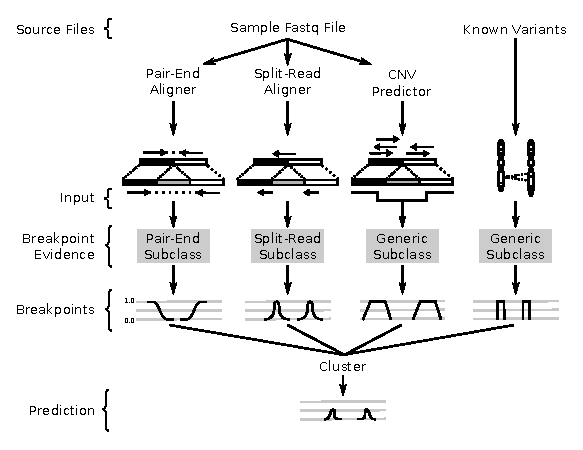
\includegraphics{Workflow.eps}
\end{figure}

\subsection{Comparison of discovery performance on simulated datasets}
In order to assess the performance of our framework, we compared our discovery
accuracy using paired-end alignments, split-read alignments, and both signals to 
three widely used SV discovery packages: Hydra \cite{Quinlan2010},
GASVPro \cite{Sindi2012} and DELLY \cite{Rausch2012b}. We created a simulated 
experimental genome by simulating 1000 deletions, duplications, insertions, 
and inversions (4000 events total) throughout chromosome 10 of the hg19 genome 
using SVsim (Faust et al, \emph{in preparation}).  For each SV event type, half
of the variants were less than 1kb and the other half were greater than 1kb (see
Methods for details).  We used the WGSIM \cite{Li2008} paired-end read 
simulator to \"sequence\" our simulated genome to 2, 5, 10, and 20 fold 
haploid coverage (Methods).

\subsection{Discovery sensitivity}
The predicted SV breakpoints from each discovery approach were compared to the
simulated breakpoints in order to measure each approach's sensitivity (Figure 2) 
and false discovery rate (FDR; Table 1). Not surprisingly, breakpoint discovery
sensitivity increases for each approach as a function of genome coverage.
Moreover, UNNAMED's sensitivity is improved when both paired-end and split-read
alignments are integrated into the probabilistic framework, as compared to 
discovery with either signal alone. In addition, UNNAMED is consistently more
sensitive than other approaches at lower coverage for all SV types. For example,
UNNAMED detects 24.5\% and 79.3\% of all deletions at 2 and 5 fold genome
coverage, whereas HYDRA, the next most sensitive approach, detects 2.9\% and
30.9\%, respectively. 

At lower coverage (i.e., 2 and 5X), UNNAMED is consistently more sensitive 
than all other approaches across all SV types. At most, UNNAMED was 
8.4 times more sensitive than the second most
sensitive approach at low coverage (UNNAMED 24.5\% vs. HYDRA 2.9\% for deletions
at 2X coverage). At worst, it was 1.2 times more sensitive for inversions at
5X coverage (UNNAMED 96.4\% vs. GASVPRO 80.8\%). At higher (20X) coverage, 
UNNAMED's sensitivity advantage persists; it ranges from 95.6\% to 97.2\% 
across all SV types, whereas HYDRA and GASVPRO range from 76.9\% to 92.8\% and
59.9\% to 91.9\%, respectively (excluding duplications for which GASVPRO is
incapable of making predictions).

Unlike the other tools compared, UNNAMED is nearly equally sensitive for 
both smaller (i.e. < 1kb) and larger (> 1kb) events. Whereas at 10X coverage,
UNNAMED detects 94.0\% and 94.2\% of deletions less and greater than 1kb, 
respectively, GASVPRO and HYDRA each have much lower sensitivity for small
variants than for large (50.7\% vs 86.2\% for HYDRA and 42.9\% and 85.3\% for
GASVPRO). This increased sensitivity is especially important given that smaller
SVs are much more common than larger events \cite{mills2011}.


\subsection{False discovery rate}
Improved SV discovery sensitivity is crucial for comprehensive characterizations
of the full spectrum of genetic variation in human genomes, yet high
sensitivity at the cost of an inflated false discovery rate (FDR) is
undesirable given the time and cost associated with pursing
the putative biological impact of spurious variation.

We compared the FDR for each SV discovery tool using the same simulated
SVs as described above (Table 1).The false discovery rate for all tools ranged 
from 0.0\% to 24.1\%. Overall, DELLY had the lowest FDR across all SV types
and genome coverage levels, yet the conservative calling comes at the cost of
reduced sensitivity compared to the other tools. While UNNAMED's FDR was 
slightly higher than GASVPRO for deletions, its FDR was consistently 
low (0.0\% - 4.6\%) across all SV types and coverage levels. In contrast, 
GASVPRO had much higher FDRs for inversions and
the FDR increased at lower coverage levels.  HYDRA had consistent FDRs across
SV types and coverage levels (0.0\% to 8.9\%), yet these rates were always 
higher than the analogous UNNAMED FDRs. These results indicate that UNNAMED's
probabilistic framework afford substantial improvements in discovery
sensitivity while maintaining low false discovery rates.



\begin{table}[h!b!p!]
\caption{False discovery rates for each SV discovery approach.}
\begin{tabular}{l|llll}
			& 20x			& 10x			& 5x			& 2x \\
\cline{2-5}
			& \multicolumn{4}{c}{Deletions} \\
\cline{1-5}
pe		&	0.014	&0.009	&0.008	&0 \\
sr      &    0.006	&0.001	&0		&0 \\
pesr    &    0.018	&0.007	&0.005	&0 \\
hydra   &    0.038	&0.01	&0.006	&0 \\
gasvpro &    0		&0		&0		&0 \\
delly pe&    0.002	&0.001	&0		&0 \\
delly sr&    0		&0		&0		&0 \\
\cline{2-5}
			& \multicolumn{4}{c}{Duplications} \\
\cline{2-5}

pe          &0.004	&0.003	&0		&0 \\
sr          &0.005	&0.002	&0.003	&0 \\
pesr        &0.007	&0.005	&0.001	&0 \\
hydra       &0.03	&0.006	&0.011	&0 \\
gasvpro     &N/A	&	N/A	&	N/A	&	N/A	 \\
delly pe    &0		&0		&0		&0.028 \\
delly sr    &0		&0		&0		&0 \\
\cline{2-5}
			& \multicolumn{4}{c}{Insertions} \\
\cline{2-5}

pe          &0.042	&0.02	&0.016	&0 \\
sr          &0.013	&0.002	&0.006	&0 \\
pesr        &0.05	&0.018	&0.009	&0 \\
hydra       &0.089	&0.034	&0.034	&0.03 \\
gasvpro     &0.242	&0.131	&0.065	&0.041 \\
delly pe    &N/A		&N/A		&N/A		&N/A \\
delly sr    &N/A		&N/A		&N/A		&N/A \\
\cline{2-5}
			& \multicolumn{4}{c}{Inversions} \\
\cline{2-5}

pe          &0.004	&0		&0		&0 \\
sr          &0.004	&0.002	&0.001	&0 \\
pesr        &0.009	&0.002	&0.002	&0 \\
hydra       &0.054	&0.013	&0.006	&0 \\
gasvpro     &0.005	&0.032	&0.082	&0.079 \\
delly pe    &0		&0		&0		&0 \\
delly sr	&0.004	&0		&0		&0 \\
\end{tabular}
\label{table:fdr}
\end{table}



\subsection{Increased breakpoint resolution}
\textbf{Include discussion of this if Ryan resolves the issue of increased
breakpoint resolution not correlating linearly with coverage.  To discuss as a 
group.}


\subsection{Benchmarks using 1000 Genomes datasets}
\textbf{Speed with 1, 2, 3, ..., 10 samples.  How many events per sample?
Need to use both PE and SR.}



%%%%%%%%%%%%%%%%%%%%%%
% Discussion
%%%%%%%%%%%%%%%%%%%%%%
\section{Discussion}
Points to make:\\
1. Mention that the framework is extensible to multiple samples. \\
2. Mention that we presented results for PE and SR, but it can be 
improved by integrating CN, existing calls, etc.  Even though our FDR for 
deletions is already quite low, we anticipate that it could be brought to ~0
by integrating CN calls from another tool.\\
3. The simulation is whole-genome unlike simulations done by other tools, 
and as such, we feel that the results have a stronger grounding in reality
than others.\\
4. The tool is easy to use, runs in reasonable times, and produces highly
sensitive and specific results.\\
5. Utility for cancer and studies of somatic instability, etc.\\



%%%%%%%%%%%%%%%%%%%%%%
% Methods
%%%%%%%%%%%%%%%%%%%%%%
\section{Methods}

We propose a breakpoint prediction framework that can accommodate multiple
classes of evidence from multiple sources in the same analysis.  To accomplish
this, we define a high-level breakpoint type that represents the consensus
breakpoint location from different pieces of evidence.  Our framework makes use
of an abstract breakpoint evidence type to define a set of functions that serve
as an interface between specific evidence subtypes (e.g., paired-end sequence
alignments and split-read mappings) and the breakpoint type.  Any class of
evidence for which these functions can be defined may be included in our
framework.  To demonstrate the applicability of this abstraction, we defined
three breakpoint evidence subtypes: paired end sequencing, split read mapping,
and a general breakpoint interface. 

Since our framework combines evidence from multiple classes, it extends
naturally to include evidence from multiple sources.  The sources that can be
considered in a single analysis may be any combination of evidence from
different samples, different evidence subclasses from the same samples, or
data sets from known genomic features.  We refer to a given data set as a
breakpoint evidence instance, and assume that each instance contains only one
evidence subtype and is from a single sample.  To help organize the results of
analysis with multiple samples or multiple instances for a single sample,
each instance is assigned an id that can be shared across instances.


\subsection{Breakpoint}

A breakpoint is a pair of genomic sequences that are adjacent in a sample genome
but not in a reference genome. Breakpoints can be detected, and their locations
predicted by various evidence classes (e.g., paired-end sequence alignments and
split-read mappings).  To support the inclusion of different evidence classes
into a single analysis, we define a high-level breakpoint type as a collection
of the evidence that corroborates the location and variety of a particular
breakpoint.  Since many evidence classes provide a range of possible breakpoint
locations, we represent the breakpoint's location with a pair of breakpoint
intervals where each interval has a a start position, an end position, and a
probability array that represents the likelihood that a given position in the
interval is one end of the breakpoint.  More formally, a breakpoint is a tuple 
$b=\langle E,l,r,w,v \rangle$ where
\begin{itemize}
\item $l$ and $r$ are left and right breakpoint intervals each with values
	$\langle s, e, p \rangle$ where
	\begin{itemize}
		\item $s$ and $e$ are the start and end genomic coordinates
		\item $p$ is a probability array where $|p|=e-s$ and $p[i]$ is the
		probability that position $s+i$ is one end of the breakpoint
	\end{itemize}
\item $E$ is set of evidence that corroborates the location and variety of a
particular breakpoint
\item $w=\sum\limits_{i=1}^{|E|} E_i.w $ cumulative breakpoint weight, were
each evidence weight represents the level of confidence in the associated
instance 
\item $v=\textsc{Deletion}|\textsc{Insertion}|\textsc{Inversion}$ is the
breakpoint variety
\end{itemize}

When a breakpoint $b$ is created from some piece of evidence, it is placed into
the set of all breakpoints $B$.  If there exits some other breakpoint $c \in B$
that intersects $b$ ($b.r$ intersects $c.r$, $b.l$ intersects $c.r$, and $b.v =
c.v$), then $b$ and $c$ are {\em merged} into interval $m$, $b$ and $c$ are
removed from $B$, and $m$ is placed into $B$.  The merged breakpoint $m$ is
defined as:
\begin{itemize}
\item $E = b.E + c.E$
\item $l.s = \max(b.l.s, c.l.s)$, $l.s = \min(b.l.e, c.l.e)$, similar for
$r.s$ and $r.e$
\item $l.p = b.l.p * c.l.p$, similar for $r.p$
\item $w = b.w + c.w$
\item $v = b.v = c.v$
\end{itemize}

Once all evidence has been considered, the breakpoints in $B$ are enumerated.
Since each genomic interval has a probability array associated with it, the
intervals may be trimmed to contain only the positions that meet some minimum
threshold (e.g., greater than 1e-10).  Some care must be taken when selecting
this value as the probabilities in this array shrink when the amount of evidence
for the breakpoint increases.


\subsection{Breakpoint Evidence}

To link the general breakpoint structured defined above and the specifics of
data like paired end sequencing alignments and split read mappings, we define
an abstract breakpoint evidence type.  This abstract type defines an interface
that allows for the inclusion of any data that can provide the following
functions:
\begin{itemize}
	\item $\textsc{is\_bp()}$ that determines if a particular
	instance of the data contains evidence of a break point
	\item $\textsc{get\_v()}$ that determines the breakpoint 
	variety (e.g., deletion, duplication, inversion, etc.)
	\item $\textsc{get\_bpi()}$ that maps the data to a pair of
	breakpoint intervals
	\item $\textsc{get\_w()}$ that represents the level of confidence
	that a specific data type is evidence of a real breakpoint
\end{itemize}

To demonstrate the applicability of this abstraction, we defined three
breakpoint evidence instances: paired end sequencing, split read mapping, and a
general breakpoint interface.  Paired end sequencing and split read mapping are
among the most frequently used data types for breakpoint detection, and the
general interface provides a mechanism to include any other breakpoint
information such as known breakpoints or output from other analysis pipelines.
As technologies evolve and our understanding of structural variations improves,
other instances can be easily added.

\subsubsection{Paired End Sequencing Alignments}

Paired end sequencing involves the fragmenting genomic DNA into roughly
uniformly sized segments, and the sequencing both ends of each segment to
produce the sequence pair $\langle x,y \rangle$.  The ends of the pair are
aligned to a reference genome $R(x)=<o,s,e>$, where $o=+|-$ indicates the
alignment orientation, and $s$ and $e$ delineate the start and end positions of
the matching sequence in the reference genome (assuming the genome is one
contiguous interval of concatenated chromosomes).  We assume that both $x$ and
$y$ align uniquely to the reference and that $R(x).s<R(x).e<R(y).s<R(y).e$.
While it is often not possible find the exact position of a sequence in the
sample genome, it is useful to refer to  $S(x)=<o,s,e>$ as the alignment of $x$
with respect to the originating sample's genome.

% is_bp
Pairs are expected to align to the reference genome with a $R(x).o=+, R(y).o=-$
orientation, and at distance $R(y).e - R(x).s$ roughly equivalent to the
fragmentation length from the sample preparation step.  Any pair that aligns an
unexpected configuration can be evidence of a breakpoint.  These unexpected
configurations include matching orientation $R(x).o = R(y).o$, alignments with
switched orientation $R(x).o=-, R(y).o=+$, and an apparent fragment length
($R(y).e - R(x).s$) that is either shorter or longer than expected.  We
estimated the expected fragment length to be the sample mean $\overline{l}$
fragment length, and the fragment length standard deviation to be the sample
standard deviation $\overline{s}$ from the set of properly mapped pairs (as
defined by the SAM spec) in the sample data set.  Given $\overline{l}$,
$\overline{s}$, and a tuning parameter $z$ to account for some variability in
the sequencing process, we can define the function $\textsc{is\_bp()}$ for the
paired end sequence alignment data type in Algorithm~\ref{is_bp}.

\begin{algorithm}[H]
    \DontPrintSemicolon
    \footnotesize
	\KwIn{Reference genome $R$, 
		  Sequence pairs $\langle x,y \rangle$,
		  expected fragment length $\overline{l}$ 
			and standard deviation $\overline{s}$,
		  tuning parameter $d$ }
    \KwOut{$\textsc{true}$ if $\langle x,y \rangle$ have an unexpected
		   alignment, otherwise $\textsc{false}$}
    \BlankLine
    \textbf{Function} $\textsc{is\_bp}$\;
	\Begin{
		\uIf{$R(x).s = R(y).s$}
			{\Return \textsc{true}\;}
		\uElseIf{$ R(y).e - R(x).s > \overline{l} + z*\overline{s}$}
			{\Return \textsc{true}\;}
		\uElseIf{$ R(y).e - R(x).s < \overline{l} - z*\overline{s}$}
			{\Return \textsc{true}\;}
		\uElse
			{\Return \textsc{false}\;}
	}
	\caption{Breakpoint evidence function that determines if a paired end
			 sequencing alignment contains evidence of a break point.}
    \label{is_bp}
\end{algorithm}

% get_v
% +- deletion or insertion
% ++ inversion
% -+ duplication
% -- inversion
The breakpoint variety for $\langle x,y \rangle$ can be inferred from the 
orientation that $x$ and $y$ align to in the reference.  If the orientations
match, then the breakpoint was caused by an inversion event, and if the
$R(x).o=-$ and $R(y).o=+$ then there was a duplication event.  When $R(x).o=+$
and $R(y).o=-$, the breakpoint variety is ambiguous between an insertion and a
deletion.  This ambiguity is also true for other types of evidence types (e.g.,
split read mappings).  While it may be possible to determine which event caused
the breakpoint in a post-processing step, breakpoint correlation is a complex
process and is beyond the scope of this framework.  Since we cannot distinguish
between the two varieties, all pairs with a $+/-$ orientation configuration are
marked as deletions.  Given $R(x).o$ and $R(y).o$, we can define the
function $\textsc{get\_v()}$ for the paired end sequence alignment
data type in Algorithm~\ref{get_v}.

\begin{algorithm}[H]
    \DontPrintSemicolon
    \footnotesize
	\KwIn{Reference genome $R$, 
		  Sequence pairs $\langle x,y \rangle$}
    \KwOut{Breakpoint variety for $\langle x,y \rangle$}
    \BlankLine
    \textbf{Function} $\textsc{get\_v}$\;
    %\textbf{Function} $\textsc{get\_v}(R(x).o,R(y).o)$\;
	\Begin{
		\uIf{$R(x).o = R(y).o$}
			{\Return \textsc{Inversion}\;}
		\uElseIf{$R(x).o = - \textbf{ and } R(y).o = +$}
			{\Return \textsc{Duplication}\;}
		\uElseIf{$R(x).o = - \textbf{ and } R(y).o = +$}
			{\Return \textsc{Deletion}\;}
	}
	\caption{Breakpoint evidence function that determines the breakpoint variety
			 for paired end sequencing alignments.}
    \label{get_v}
\end{algorithm}

% get_bpi
To map $\langle x,y \rangle$ to breakpoint intervals $l$ and $r$, the ranges of
possible breakpoint locations must be determined and probabilities assigned to
each position in those ranges.  By convention, $x$ maps to $l$ and $y$ to
$r$, and for the sake of brevity we will focus on $x$ and $l$ since the same
process applies to $y$ and $l$.  Assuming that a single breakpoint exists
between $x$ and $y$, then the sign of $x$ determines if $l$ will be upstream
or downstream of $x$.  If the $R(x).s=+$, then the breakpoint interval begins
after $R(x).e$ (downstream), otherwise the interval ends before $R(x).s$
(upstream).  
%To account for variance in the alignment of $x$, we extend the breakpoint by
%to $R(x).e - v_a$ if $R(x).s=+$ and $R(x).s + v_a$ if $R(x).s=-$,
%where $v_a$ is a turning parameter.

The length of each breakpoint interval is proportional to the expected fragment
length $\overline{l}$ and standard deviation $\overline{s}$.  Since we assume
that only one breakpoint exists is between $x$ and $y$, and that it is unlikely
that the distance between the ends of a pair in the sample genome ($S(y).e -
S(x).s$) is greater than $\overline{l}$, then it is unlikely that one end of the
breakpoint is at a position greater than $R(x).s + \overline{l}$, assuming that
$R(x).o=+$. If $R(x).o=-$, then it is unlikely that a breakpoint is at a
position less than $R(x).e - \overline{l}$.  To account for variability in the
fragmentation process, we extend the breakpoint to 
$R(x).e + \overline{l} + v_f*\overline{s}$ when $R(x).o=+$, and 
$R(x).s - (\overline{l} + v_f*\overline{s})$ when $R(x).o=-$, 
where $v_f$ is a tuning parameter.  

The probability that a particular position $i$ in the breakpoint interval $l$ is
part of the actual breakpoint can be estimated by the probability that $x$ and
$y$ span that position in the sample. For $x$ and $y$ to span $i$, the fragment
that produced $\langle x,y \rangle$ must be longer than then distance from the
start of $x$ to $i$, otherwise $y$ would occur before $i$ and $x$ and$y$ would
not span $i$ which is a contradiction.  The resulting probability is 
$P(S(y).e - S(x).s > i - R(x).s)$ if $R(x).o=+$, and 
$P(S(y).e - S(x).s > R(x).e - i)$ if $R(x).o=-$.
While we cannot directly measure the sample fragment length ($S(y).e - S(x).s$),
we can estimate its distribution by constructing a frequency-based cumulative
distribution $D$ of fragment lengths from the same sample that was used to find
$\overline{l}$ and $\overline{s}$, where $D(j)$ gives the proportion of the
sample with fragment length greater than $j$.

\begin{algorithm}[H]
    \DontPrintSemicolon
    \footnotesize
	\KwIn{Reference genome $R$, 
		  One end of a sequence pair $z$,
		  expected fragment length $\overline{l}$ 
		  and standard deviation $\overline{s}$,
		  tuning parameter $v_f$,
		  fragment length cumulative distribution $D$}
    \KwOut{One end of a breakpoint interval $t$}
    \BlankLine
    \textbf{Function} $\textsc{get\_one\_bpi}$\;
		%$\textsc{get\_one\_bpi}(R,z,\overline{l},\overline{s},v_f,D)$\;
	\Begin{
		\uIf{$R(x).o = +$} {
			$t.s \gets R(z).e$\;
			$t.e \gets R(z).e + \overline{l} + v_f*\overline{s}$\;
			\For{$i = 1 \to ( t.e - t.s ) $} {
				$t.p[i] \gets D(j)$\;
			}
		}
		\uElse {
			$t.e \gets R(z).s$\;
			$t.s \gets R(z).s - (\overline{l} + v_f*\overline{s})$\;
			\For{$i = 1 \to ( l.e - l.s ) $} {
				$t.p[(t.e-t.s) - i] \gets D(j)$\;
			}
		}	
		\Return $t$\;
	}
	\caption{Breakpoint evidence function that maps one end of a sequence pair
			to one end of a breakpoint interval.}
    \label{get_one_bpi}
\end{algorithm}

\begin{algorithm}[H]
    \DontPrintSemicolon
    \footnotesize
	\KwIn{Reference genome $R$, 
		  Sequence pair $\langle x,y \rangle$,
		  expected fragment length $\overline{l}$ 
		  and standard deviation $\overline{s}$,
		  tuning parameter $v_f$,
		  fragment length cumulative distribution $D$}
   \KwOut{Breakpoint intervals $l$ and $r$}
    \BlankLine
    \textbf{Function} $\textsc{get\_bpi}$\;
		%(R,\langle x,y \rangle,\overline{l},\overline{s},v_f,D)$\;
	\Begin{
		$l \gets \textsc{get\_one\_bpi}(R,x,\overline{l},\overline{s},v_f,D)$\;
		$r \gets \textsc{get\_one\_bpi}(R,y,\overline{l},\overline{s},v_f,D)$\;
		\Return $l,r$
	}
	\caption{Breakpoint evidence function that maps a sequence pair alignment to
			a breakpoint interval.}
    \label{get_bp}
\end{algorithm}

% get_w

The weight of each sequcence pair is an input parameter $v_w$.

\subsubsection{Split Read Alignments}

A split read alignment is a single DNA fragment $X$ that does not uniquely align
to the reference genome, but contains a contiguous ordered set of substrings
$(x_1, x_2, \dots, x_n)$ where $X=x_1x_2\dots x_n$, each substring aligns
uniquely to the reference $R(x_i)=\langle o,s,e \rangle$, and adjacent
substrings align to non-adjacent location in the reference genome
$R(x_{i}).e \neq R(x_{i+1}).s + 1$ for $1\leq i \leq n-1$. A single split read
alignment maps to a set of adjacent split-read sequence pairs 
$(\langle x_1 , x_2 \rangle, \langle x_2, x_3 \rangle, \dots ,
\langle x_{n-1},x_n \rangle)$, and each pair is considered individually.

% is_bp
By definition, a split-read mapping is evidence of a breakpoint and therefore
the function $\textsc{is\_bp()}$ trivially returns $\textsc{true}$.

% get_v
Both orientation and mapping location must be considered to infer the breakpoint
variety for $\langle x_i,x_{i+1} \rangle$.  When the orientations match
$R(x_{i}).o=R(x_{i+1}).o$, the event was either a deletion or
a duplication.  Assuming the $R(x_{i}).o=R(x_{i+1}).o=+$, 
$R(x_{i}).s<R(x_{i+1}).s$ indicates a gap caused by a deletion and 
$R(x_{i}).s>R(x_{i+1}).s$ indicated a repeated sequenced caused by a
duplication.   These observations are flipped when orientations
$R(x_{i}).o=R(x_{i+1}).o=-$.  Similar to paired end alignments, we do mark any
breakpoint as an insertions since we cannot distinguish between deletions and
insertions.  When the orientations do not match $R(x_{i}).o \ne R(x_{i+1}).o$,
the event was an inversion and the mapping locations do not need to be
considered.  Given $R(x_i).o$, $R(x_i).s$, $R(x_{i+1}).o$, and $R(x_{i+1}).s$,
we can define the function $\textsc{get\_v()}$ for the paired end sequence
alignment data type in Algorithm~\ref{get_v_sr}.

\begin{algorithm}[H]
    \DontPrintSemicolon
    \footnotesize
	\KwIn{Reference genome $R$, 
		  Sequence pairs $\langle x,y \rangle$}
    \KwOut{Breakpoint variety for $\langle x,y \rangle$}
    \BlankLine
    \textbf{Function} $\textsc{get\_v}$\;
	\Begin{
		\uIf{$R(x_i).o \ne R(x_{i+1}).o$}
			{\Return \textsc{Inversion}\;}
		\uElseIf{$R(x_i).o=R(x_{i+1}).o=+ \textbf{ and } R(x_i).s<R(x_{i+1}).s$}
			{\Return \textsc{Deletion}\;}
		\uElseIf{$R(x_i).o=R(x_{i+1}).o=- \textbf{ and } R(x_i).s>R(x_{i+1}).s$}
			{\Return \textsc{Deletion}\;}
		\uElseIf{$R(x_i).o=R(x_{i+1}).o=+ \textbf{ and } R(x_i).s>R(x_{i+1}).s$}
			{\Return \textsc{Duplication}\;}
		\uElseIf{$R(x_i).o=R(x_{i+1}).o=- \textbf{ and } R(x_i).s<R(x_{i+1}).s$}
			{\Return \textsc{Duplication}\;}
	}
	\caption{Breakpoint evidence function that determines the breakpoint variety
			 for split-read alignments.}
    \label{get_v_sr}
\end{algorithm}

% get_bpi
The possibility of errors in the sequencing and alignemnt processes create some
ambiguity in the exact location of the breakpoint associated with a split-read
sequence pair.  To acount for this, each pair $\langle x_i, x_{i+1} \rangle$
maps to two breakpoint intervals $l$ and $r$ centered at the split. The 
probability vectors $l.p$ and $r.p$ are highest at the midpoint and
exponentially decreaseing toward their edges.  The size of this interval is a
configurable parameter $v_s$ and is based on the quality of the sample under
consideration and the specificity of the alignment algorithm used to map the
sequences to the reference.

Depending the breakpoint variety, the intervals $l$ and $r$ are centered on
either the start or the end of $R(x_i)$ and $R(x_{i+1})$.  When the breakpoint
is a deletion $l$ is centered at $R(x_i).e$ and $r$ at $R(x_{i+1}).s$, and when
the breakpoint is a duplication $l$ is centered at $R(x_i).s$ and $r$ at
$R(x_{i+1}).e$.  If the breakpoint is an inversion, $l$ and $r$ are both 
centered ether at the start positions or end positions of $R(x_i)$ and
$R(x_{i+1})$, respectivly.  Assuming that $R(x_i).s<R(x_{i+1}).s$, if
$R(x_i).o=+$ then $l$ and $r$ are centered at $R(x_i).e$ and  $R(x_{i+1}).e$,
otherwise they are centered at $R(x_i).s$ and  $R(x_{i+1}).s$.  If
$R(x_i).s>R(x_{i+1}).s$, then the conditions are swapped.


\begin{algorithm}[H]
    \DontPrintSemicolon
    \footnotesize
	\KwIn{Reference genome $R$, 
		  Split-read pair $\langle x_i,x_{i+1} \rangle$,
		  tuning parameter $v_s$,
		  breakpoint variety $v$ }
   \KwOut{Breakpoint intervals $l$ and $r$}
    \BlankLine
    \textbf{Function} $\textsc{get\_bpi}$\;
	\Begin{
		$l_c \gets NULL$	
		$r_c \gets NULL$	

		\uIf{$v = \textsc{Inversion}$} {

			\uIf{$R(x_i).s<R(x_{i+1}).s$} {
				\lIf{$R(x_i).o=+$}
					{$l_c\gets R(x_i).e,r_c\gets R(x_{i+1}).e$}\;
				\lElse {$l_c\gets R(x_i).s,r_c\gets R(x_{i+1}).s$}\;
			} \Else {
				\lIf{$R(x_i).o=+$}
					{$l_c\gets R(x_i).s,r_c\gets R(x_{i+1}).s$}\;
				\lElse
					{$l_c\gets R(x_i).e,r_c\gets R(x_{i+1}).e$}\;
			}

		}
		\lElseIf{$v = \textsc{Deletion}$} 
			{$l_c\gets R(x_i).e,r_c\gets R(x_{i+1}).s$}\;
		\lElseIf{$v = \textsc{Duplication}$} 
			{$l_c\gets R(x_i).s,r_c\gets R(x_{i+1}).e$}\;

		$l.s\gets l_c - v_s, l.e\gets l_c + v_s$\;
		$r.s\gets r_c - v_s, r.e\gets r_c + v_s$\;

		$\lambda = \log(1e-10)/-v_s$\;
		\For{$i = 1 \to v_s $} {
			$l.p[i] \gets r.p[i] \gets \exp^{-\lambda(v_s - i)}$
		}
		\For{$i = v_s \to 2*v_s $} {
			$l.p[i] \gets r.p[i] \gets \exp^{-\lambda(i - v_s)}$
		}
	
		\Return $l,r$
	}
	\caption{Breakpoint evidence function that maps a sequence pair alignment to
			a breakpoint interval.}
    \label{get_bp_sr}
\end{algorithm}

% get_w

The weight of each sequcence pair is an input parameter $v_w$.

\subsubsection{Generic Evidence}

The generic evidence subclass provides a mechanism to include a wide variety of
data, from known varients to tool output.

two example, known vairents and cnv


% is_bp
% type
% get_bp
\section{Simulation Results}
\section{TCGA Results}

\bibliographystyle{plain}
\bibliography{recomb}

\end{document}
